% vim: spelllang=en spell textwidth=120
\documentclass[deska]{subfiles}
\begin{document}

\chapter{Server part of deska}
\label{sec:deska-server}

\begin{abstract}
Talk about server part of deska application. Deska server application and deska database.
\end{abstract}

\section{Design}
Server part of deska application can be devided into two parts. The deska-server and deska database.
Deska-server is python application, that runs for every user, listen for the commands from deska-cli (see dbapi protocol).
Main work is to load json data, call corresponding stored function, and return the answer to deska-cli.
There are some special functions (freezeChangeset, showConfigDiff etc.) that are not implemented by deska db, but the server itselfs.

\subsection{Deska server}
FIXME: about deska server configuration generators & some tricks (maybe) in deska-server to explain.

\subsection{Deska database}
Deska database is devided into several parts. Every part is in special db schema. 

User defined schema, that contains user modules/tables with all indexes and triggers, is contained in schema production. After each commit, into these tables are copied resolved data, all user defined triggers and checks are run, so that contained data are checked as it was specified in modules definition.

In history schema are stored all tables used for history tracking, work in temporary changeset. Every kind (module i one kind, or two - if it is templetized) has one table here, with columns copied from production table and some more added for history tracking.

For every kind there is bunch of stored procedures, which are used for manipulation with data in history tables. For example for kind vendor, there are functions like vendor\_add, vendor\_set\_(all attributes), vendor\_del ….
These functions, created by sql generator are stored in genproc schema.

The deska schema is used for functions and another objects that needed from many functions, but are not generated. There are also functions for manipulationg with changesets and versions.
But not the tables including data about changesets and versions. These tables are in versioning schema.

Functions which are called by deska-server are in json schema.

Schema testing stores some functions used by tests, these functions are not needed for deska database at all (except running tests).
\begin{figure}[h]
	\centering
	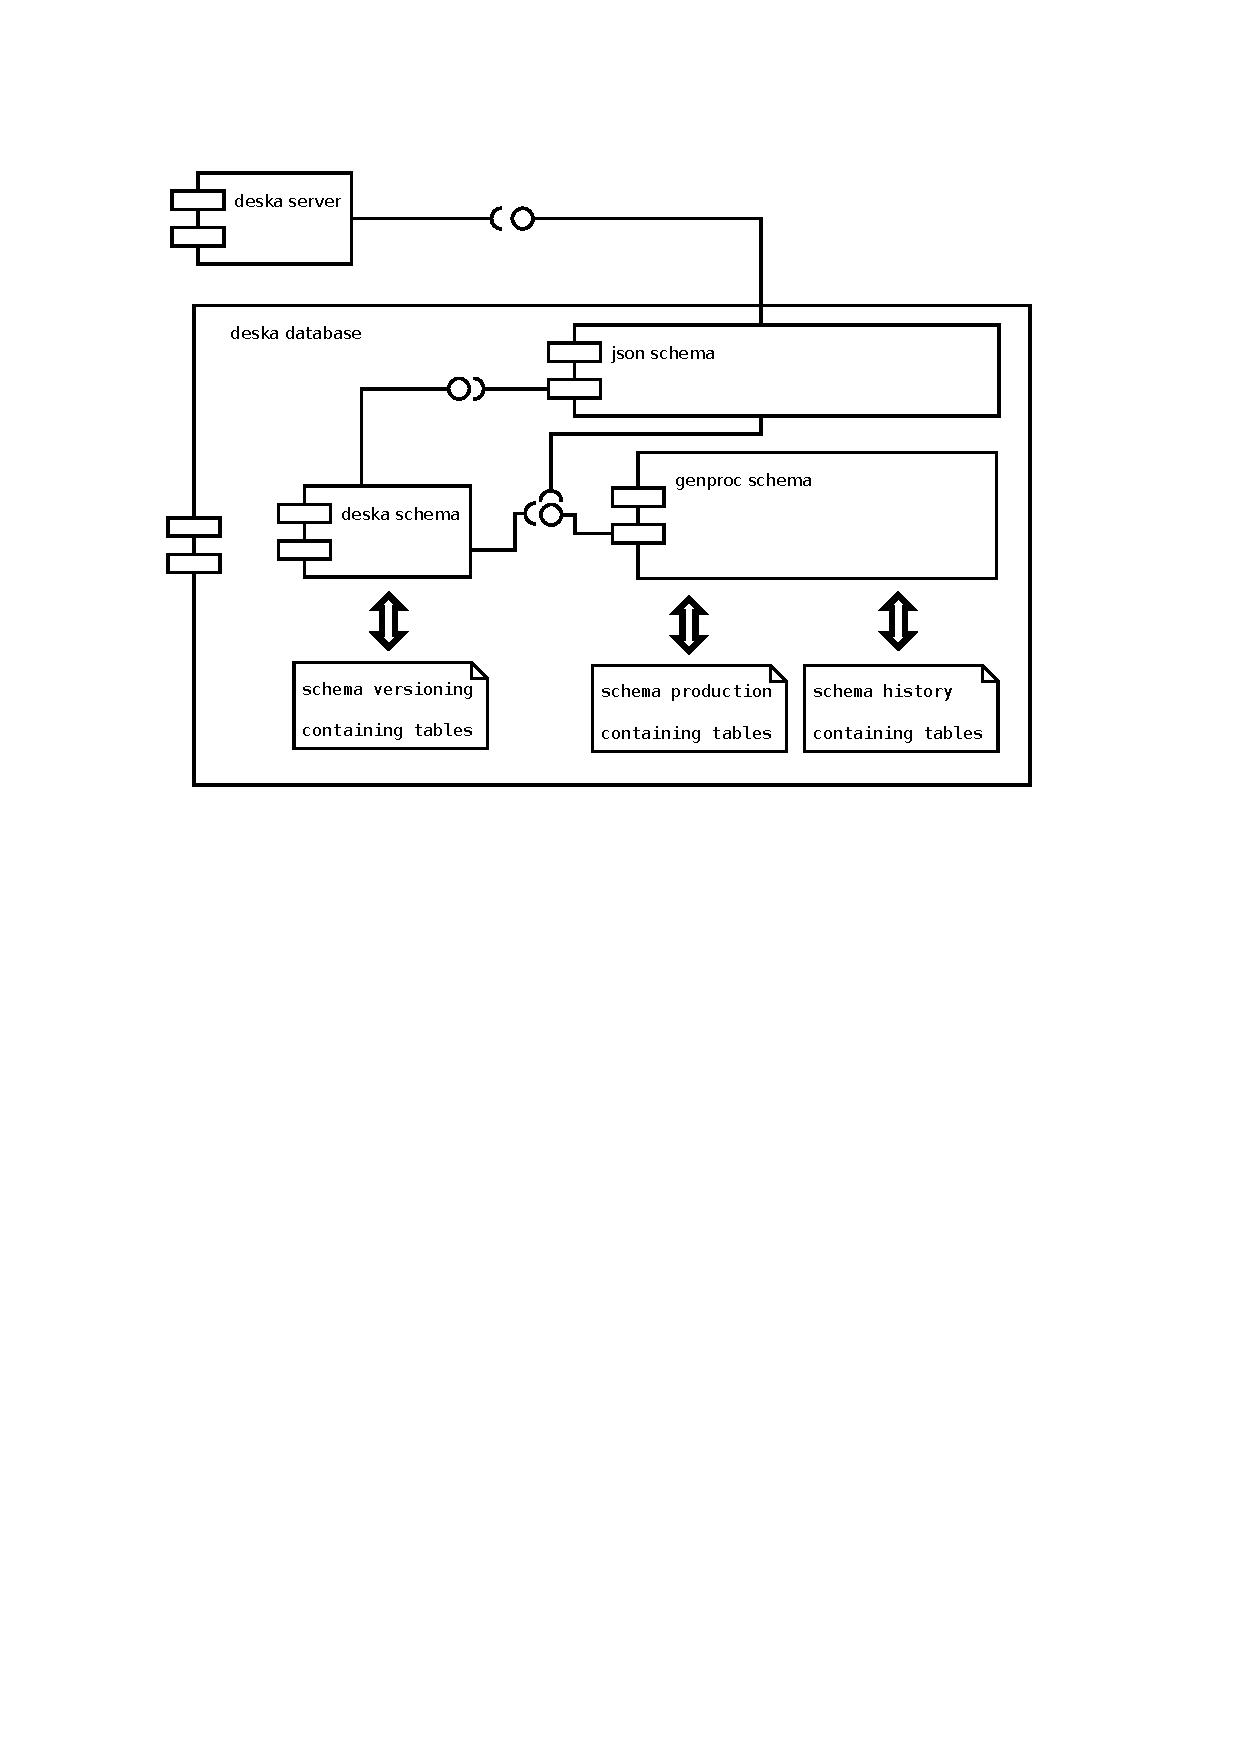
\includegraphics[trim=28mm 170mm 30mm 28mm]{img-deska-server-components.pdf}
	\caption{Deska server components}
\end{figure}

The philosophy of this desing is, that deska-server calls function in json schema (deska user is db role, for normal user, and it has rights only to run functions in schama json). Functions in json schema are using functions from deska schema (for work with versioning tables) or functions from genproc schema (for work with history and production tables).

\subsection{Filters}

\subsubsection{Function of filter}

Some functions in json schema have parametr filter. It is in json fomrat, see dbapi protocol for more info.
This filter is implemented in filter.py file in class filter. It support creation of WHERE part, that is added to select statement called from functions with filter parametr, and also JOIN part which is used in the same way.

As we said, some kind specific function is determined, for example hardware\_get\_version() (as data source for multipleObjectData function). There for some "SELECT [columns definition here] FROM hardware\_get\_version() AS hardware" is created. But if there is used some filter, we have to add WHERE part to this select. If the filter ask for some attribute of another kind, for example name of host which runs on the hardware, even JOIN part must be added. For it, there are Filter class methods getWhere and getJoin. 

Here it must be said, that you can join only kind (in fact it is some view on table, implemented as a function), which is in some relation with kind we operate with. The filter works with all relations and both directions presented in deska, but not transitively.

\subsubsection{Implementation}

The filters are created from two classes. Filter, which contains information about filter itself, parse the filter and creates
the JOIN and WHERE part of sql select statement. And Condition class, which stores information about each condition in filter, and provides
one sql part of WHERE part. It takes information from condition definition in filter parametr, and also from relation information provided
in generated.py file output of generators.

\subsection{Error handling}
Here we try to explain work with exception in deska database/ server. Postgre sql functions can RAISE exception with given message and sqlstate.
This sqlstate is like number of error. We use this to split posible exceptions into some category - exception types. Exception in database is
every unexpected or “bad” thing that occures. It can be run time error as well as contraint violation, or exception thrown explicitly by RAISE.

Psycopg used in deska-server to perform actions in db, has no good way to get sqlstate of exception, whích is used to determine exception type.
This is reason to catch maximum number of exception inside the database (in json schema part), so that exception type can be determined.

Functions in json schema catches all exceptions and transform it into json - see format of this execption in dbapi specification.
For this transformation DeskaException class is used. It has constructor, with Postgresql.dberr, which is structure that contains exception
message, and sqlstate. We use this information to determine exception type - class contains typeDict - dictionary {sqlstate: exceptionType}.
Finally this function has json method, which takes name on the function, in which error occures and creates exception in json format.

\end{document}
